\documentclass[a4paper,12pt]{scrartcl}
\usepackage[utf8]{inputenc}
\usepackage{amsmath}
\usepackage{bbold}

\usepackage{graphicx}
\usepackage{caption}
\usepackage{subcaption}
\usepackage[left=3cm,right=3cm,top=3.5cm,bottom=3.5cm]{geometry}
\usepackage{pgfplots,pgfplotstable}
\usepackage{tikz}
%\usetikzlibrary{positioning, fadings, through}
\usepackage{fancyhdr}
\usepackage[locale=DE,output-decimal-marker={.}]{siunitx}
\sisetup{separate-uncertainty, per-mode=fraction,}
\usepackage{here}
\usepackage{hyperref}

\usepackage{setspace}
\onehalfspacing
\usepackage{comment}

\usepackage{circledsteps}

% Default fixed font does not support bold face
\DeclareFixedFont{\ttb}{T1}{txtt}{bx}{n}{12} % for bold
\DeclareFixedFont{\ttm}{T1}{txtt}{m}{n}{12}  % for normal

% Custom colors
\usepackage{color}
\definecolor{deepblue}{rgb}{0,0,0.5}
\definecolor{deepred}{rgb}{0.6,0,0}
\definecolor{deepgreen}{rgb}{0,0.5,0}

\usepackage{listings}

% Python style for highlighting
\newcommand\pythonstyle{\lstset{
numbers=left,
language=Python,
basicstyle=\ttm,
otherkeywords={self},             % Add keywords here
% keywordstyle=\ttb\color{deepblue},
emph={MyClass,__init__},          % Custom highlighting
emphstyle=\ttb\color{deepred},    % Custom highlighting style
stringstyle=\color{deepgreen},
frame=tb,                         % Any extra options here
showstringspaces=false            % 
}}


% Python environment
\lstnewenvironment{python}[1][]{
\pythonstyle
\lstset{#1}
}{}

% Python for external files
\newcommand\pythonexternal[2][]{{
\pythonstyle
\lstinputlisting[#1]{#2}}}

% Python for inline
\newcommand\pythoninline[1]{{\pythonstyle\lstinline!#1!}}


\usepackage{booktabs}
\usepackage{multirow}
\usetikzlibrary{external}
\tikzexternalize[prefix=tikz/]

\pgfplotsset{compat=newest,
    tick label style={font=\small},
    label style={font=\small},
    legend style={font=\footnotesize}
    }
    
\tikzset{every mark/.append style={scale=0.3}}
\tikzset{>=stealth}
\usepackage{acronym}
\newlength{\plotheight}
\newlength{\plotwidth}
\newlength{\imgheight}
\setlength{\plotwidth}{14cm}
\setlength{\plotheight}{8cm}


\newcommand{\titel}{Finite Difference Time Domain}
\usepackage{fancyhdr}
\fancyhf{}
\pagestyle{fancy}
\cfoot{\thepage}
\fancyhead[L]{\leftmark}
\fancyhead[R]{\thepage}

\subject{Report}
\title{\titel}
\author{\large{Martin \textsc{Aleksiev}, Felix \textsc{Wechsler}, Mei \textsc{Yunhao}, Mingxuan \textsc{Zhang}}\\  \large{Group 3}}
\date{\large{\today}}
\publishers{\vspace{5.5cm}Abbe School of Photonics\\
            Friedrich-Schiller-Universität Jena}


\newcommand\todo[1]{\textcolor{red}{\textbf{TODO: #1}}}

%proper Integral typsetting
\newcommand{\dt}{\, \mathrm{d}t}
\newcommand{\dd}{\mathrm{d}}

\newcommand\ff[1]{ \mathbf #1(\mathbf r, \omega)}
\newcommand\lap{\mathop{{}\bigtriangleup}\nolimits}

\usepackage[%
  backend=biber,
  url=false,
  style=alphabetic,
  % citestyle=authoryear,
  maxnames=4,
  minnames=3,
  maxbibnames=99,
  giveninits,
uniquename=init]{biblatex}

\addbibresource{references.bib}
\pgfkeys{/csteps/inner color=transparent , /csteps/outer color=black}


%indentation to 0
\setlength\parindent{0pt}
\begin{document}
    \maketitle
	\thispagestyle{empty}
	\newpage
	\setcounter{page}{1}
	\tableofcontents

\newpage
\section{Introduction}
    In this report we present the basics of the Finite Difference Time Domain numerical method.
    This method allows to fully solve Maxwell's equation without any approximations.
    After providing the physical background, we show how to implement the solution with 
    a Yee-grid and show results for the simulation of a pulsed beam in a 1D and 3D case.

\section{Physical Background}
   The physical basics are Maxwell's equation (MWEQ):
   \begin{align}
       \nabla \times \ff{E} &= - \frac{\partial \ff B} {\partial t}\\
        \nabla \times \ff{H} &=  \frac{\partial \ff D} {\partial t} + \ff j \\
        \nabla \cdot \ff D &= \rho(\mathbf r , t)\\
        \nabla \cdot \ff B &= 0
   \end{align}
   with $\ff E$ being the electric field, $\ff H$ the magnetic field, $\ff D $ the dielectric flux density,
   $\ff B$ the magnetic flux density, $\ff P$ the dielectric polarization, $\rho (\mathbf{r}, t)$ the external charge density and
   $\ff j$ the macroscopic current density.
   In an isotropic, dispersionless and non-magnetic media we furthermore obtain the following material equations:
   \begin{align}
       \ff D &= \epsilon_0 \epsilon(\mathbf r) \ff E\\
       \ff B &= \mu_0 \ff H
   \end{align}
   In this case, MWEQ can be expressed as:
    \begin{align}
        \nabla \times \ff{E} &= - \mu_0 \frac{\partial \ff H} {\partial t}
        \label{eq:final_}\\
        \nabla \times \ff{H} &=  \epsilon_0 \epsilon(\mathbf r) \frac{\partial \ff E} {\partial t} + \ff j 
        \label{eq:final}
    \end{align}
   \ref{eq:final_} and \ref{eq:final} are the final equations we are going to solve in the next sections.
   
 \section{Numerical Implementation}
    To solve the equations, we can explicitly express one of the cross products:
    \begin{equation}
        \frac{\partial E_x}{\partial t} = \frac1{\epsilon_0 \epsilon(\mathbf r)} \left( \frac{\partial H_z}{\partial y} -  \frac{\partial H_z}{\partial y} - j_x \right)
    \end{equation}
    Using a second order central-difference scheme for both the time and spatial
    derivatives we obtain the resulting equations for a 1D case:
    \begin{align}
        E_x^{n+1} &= E_x^{n-1} +  \frac1{\epsilon_0 \epsilon} \frac{\Delta t}{\Delta x} (H_{x+\Delta x}^n - H_{x-\Delta x}^n - j_x)\\
        H_y^{n+1} &= H_y^{n-1} +  \frac1{\mu_0} \frac{\Delta t}{\Delta x} (E_{x+\Delta x}^n - E_{x-\Delta x}^n)
    \end{align}
    It can be observed that $E$ and $H$ are updated in an alternating way.
    Therefore, one can introduce the Yee grid with a Leapfrog time stepping scheme.
    A visual representation of the scheme can be see in \autoref{fig:yee}.
    \begin{figure}[H]
        \centering
        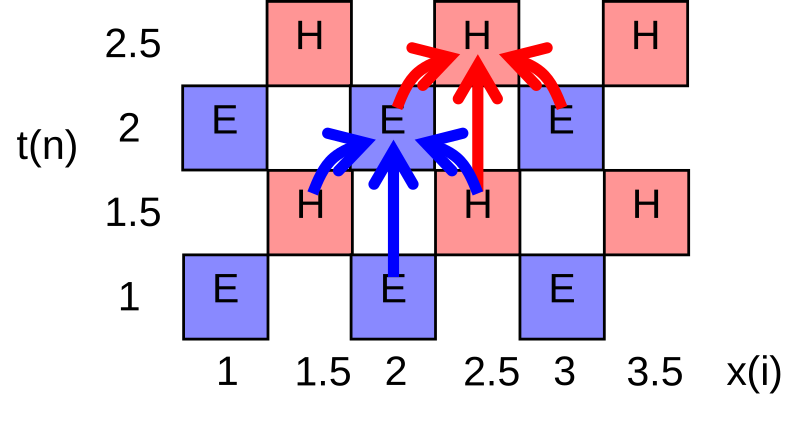
\includegraphics[width=.5\textwidth]{figures/yee.png}
        \caption{Yee grid with a Leapfrog time stepping. Figure taken from \cite{lecture}.}
        \label{fig:yee}
    \end{figure}
    One can finally express the equations in the Yee grid as:
        \begin{align}
        E_i^{n+1} &= E_i^{n} +  \frac1{\epsilon_0 \epsilon} \frac{\Delta t}{\Delta x} (H_{i+0.5}^{n+0.5} - H_{i-0.5}^{n+0.5} - \Delta x \cdot j_{i+0.5}^{n+0.5})\\
        H_{i+0.5}^{n+1.5} &= H_{i+0.5}^{n+0.5} +  \frac1{\mu_0} \frac{\Delta t}{\Delta x} (E_{i+1}^{n+1} - E_{i}^{n+1})
    \end{align}
    The current source $j_z$ is defined using a delta distribution, meaning it is zero everywhere, except for one spatial position. It has a gaussian temporal envelope and is described by the following equation:
    \begin{align}
        j_z &= \exp\left(-2\pi ift\right) \cdot \exp\left(-\frac{(t-t_0)^2}{\tau ^2}\right)  
    \end{align}
    The fields are calculated for different spatial positions using indexing and for different times via a for loop. The $E$-field is assumed to be a perfect conductor at the boundaries and as a result, those values are set to zero. \\
    For the 3D case, there are a fer aditional considerations taken. The tangential E-fields and normal H-fields are stored in arrays of size $N$, whereas the tangential $H$-fields and normal E-fields are stored in $N-1$ size arrays. This is due to the Yee grid being in 3 dimentions and having integer and fractional indices. Due to these indices, the permittivity must be aslo interpolated. 
    A for loop is used to calculate the fields for different times, analogously to the 1D case with the addition of saving the calculated fields every output step, which we choose. These fields are interpolated so that we have all fields on a common grid in space and time.

% \newpage
\section{Results}
    In this section we present some results of the simulations.
    \autoref{fig:1Dres} shows the electric and magnetic field for 
    a current being injected into the space.
    We observe that two pulses are propagating in different direction.
    \begin{figure}[H]
        \begin{subfigure}{.5\textwidth}
            \centering
            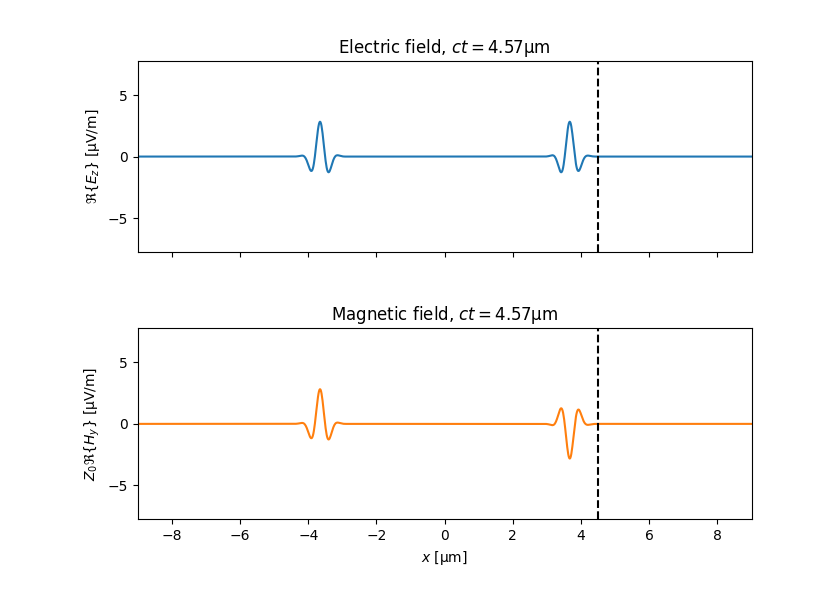
\includegraphics[width=\textwidth]{figures/Figure_1D1.png}
            \caption{$ct = \SI{4.57}{\micro\meter}$}
            \label{fig:1Dl}
        \end{subfigure}
        \begin{subfigure}{.5\textwidth}
            \centering
            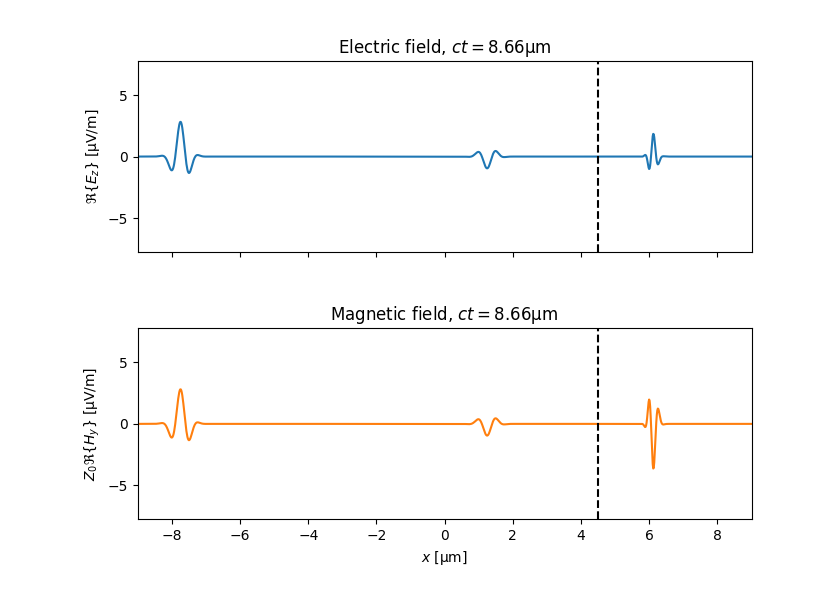
\includegraphics[width=\textwidth]{figures/Figure_1D2.png}
            \caption{$ct = \SI{8.66}{\micro\meter}$}
            \label{fig:1Dr}
        \end{subfigure}
        \caption{Electric and magnetic field for the 1D problem.}
        \label{fig:1Dres}
    \end{figure}
    In \autoref{fig:1Dr} we can observe that in the medium on the right hand side of the dashed line (higher $\epsilon$) the pulse is
    compressed. This is due to the slower group velocity. Furthermore the amplitude is reduced. We notice that a third pulse appeared due to reflection according to Fresnel reflection laws.
    
    In \autoref{fig:3Dres} we can see the electric field propagating
    in radial manner starting at the center. In the center we injected a current guided in z direction. 
    \begin{figure}[H]
        \begin{subfigure}{.5\textwidth}
            \centering
            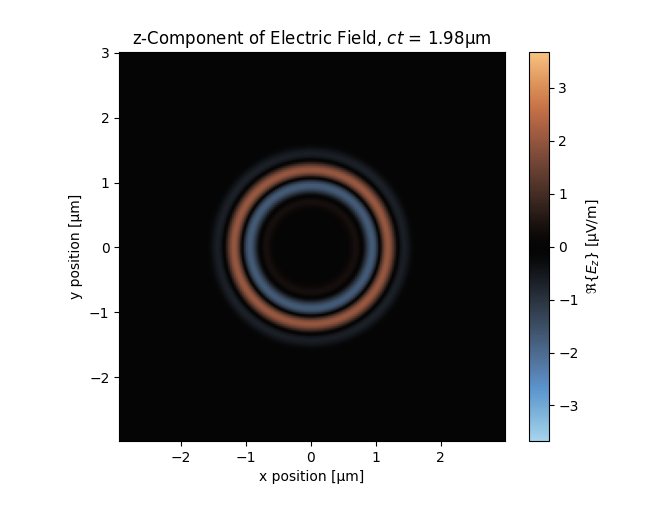
\includegraphics[width=\textwidth]{figures/3D-Ez.png}
            \caption{Electric field of the z-component}
            \label{fig:3Dl}
        \end{subfigure}
        \begin{subfigure}{.5\textwidth}
            \centering
            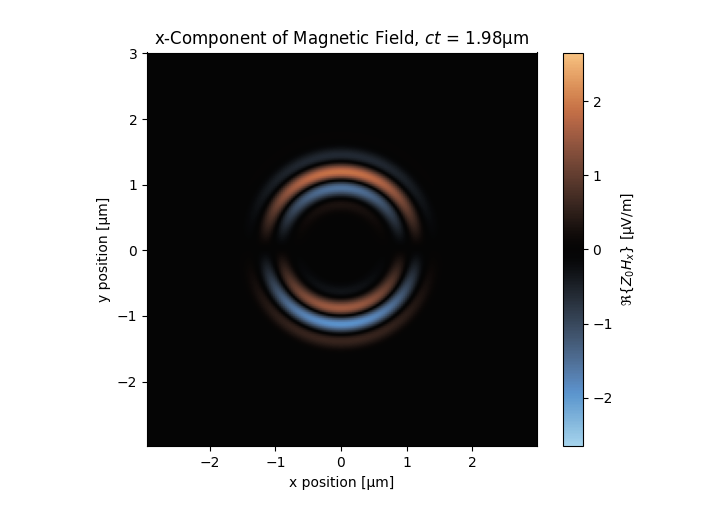
\includegraphics[width=\textwidth]{figures/3D-Hx.png}
            \caption{Magnetic field of the x-component}
            \label{fig:3Dr}
        \end{subfigure}
        \caption{Cross section at of the 3D field with a current pulse originating from the center.}
        \label{fig:3Dres}
    \end{figure}
    The electrical field is radial symmetric, the magnetic field not.
    This is due to the reason that we displaying the $x$ component of the $H$ field. And due to the divergence condition the $x$ component 
    must be 0 in the $x$ direction.
    
    
    \subsection{Computational Performance}
        In this section we provide some data for the computational performance.
        Our setup for all measurements was Python 3.8.2, SciPy 1.3.2, NumPy 1.17.3 and a Intel(R) Core(TM) i7-7600U CPU @ 2.80GHz.
        The example scripts are attached to this report.
        In \autoref{tab:res} we can see the computational time
        for different datatypes and for 1D and 3D. Obviously 1D is much faster than the full 3D approach.
        \begin{table}[h]
            \centering
            \setstretch{1.5}
            \begin{tabular}{l r}
               &  Total time needed in \si{\second}  \\
               \hline
                1D, single precision &  $0.136\pm 0.001$ \\
                1D, double precision &  $0.187\pm 0.001$ \\
                \hline
                3D, single precision &  $5.11\pm 0.05$ \\
                3D, double precision &  $6.413\pm 0.02$  \\
            \end{tabular}
            \caption{Results for the computing time}
            \label{tab:res}
        \end{table}
        However, we can see that the datatype does not have a significant
        impact on the time needed. This is due to the reason that Python is an interpreted language and therefore source code relying on for loops is usually slow. In Python this cannot circumvented since the core functions within the for loop are rather trivial and do not rely on external functions call taking most of the time.
        For a better performance once should use a compiled language or modern approaches like Julia.
        
    \subsection{Convergence Rate}
        In this part we show results of the convergence rate for different spatial and time resolutions.
        For a quick estimation we compare the fields to higher sampled numerical versions instead of an analytical one.
        In our source code the spatial and temporal sampling are connected:
        \begin{equation}
            \Delta t = \frac{\Delta r}{2 c}
        \end{equation}
        Therefore by varying the spatial sampling we also vary the temporal one.
        \begin{figure}[H]
            \centering
            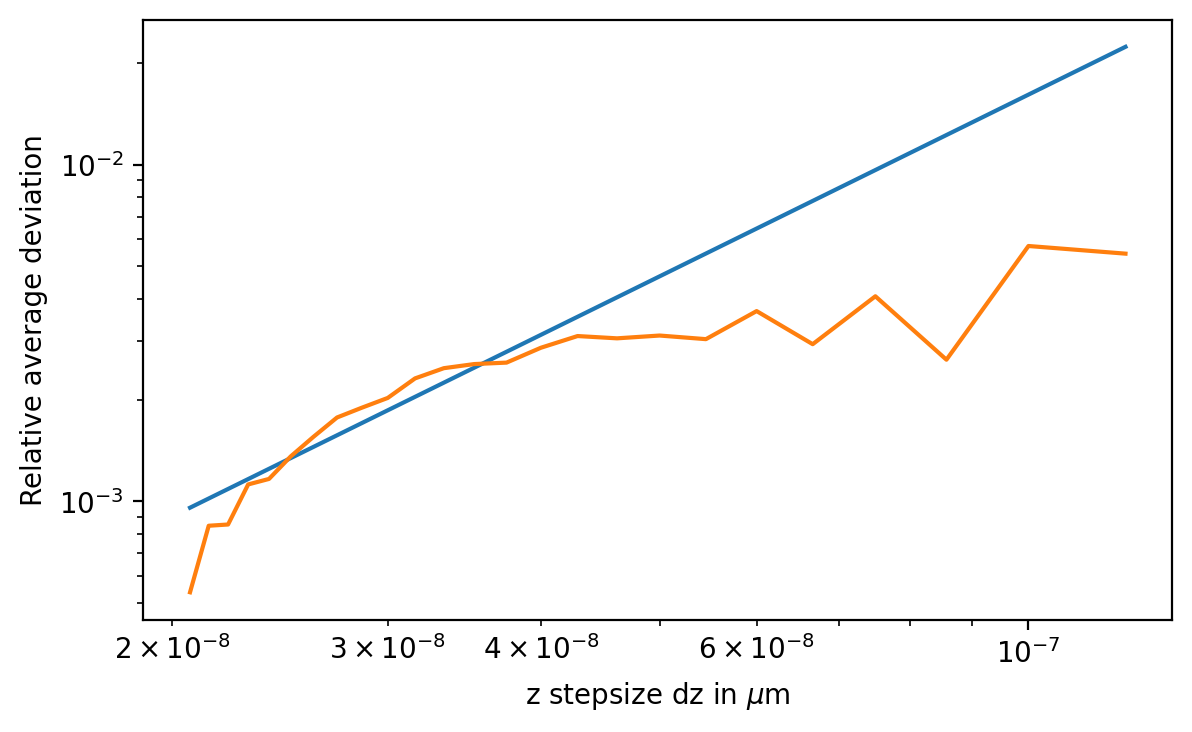
\includegraphics[width=.8\textwidth]{figures/index.png}
            \caption{Convergence behaviour with different $\Delta r$ sampling.}
            \label{fig:conv}
        \end{figure}
        In \autoref{fig:conv} we can see the convergence behaviour of the FDTD. Note that this plot is double logarithmic.
        The slope of the blue curve is $\SI{1.79\pm0.16}{\per\micro\meter}$. The theoretical convergence of the algorithm is 2, so our measured values comes close to that one.
        The reason for the deviation could be the boundary handling and artificats due to the fact that we comparing against a numerical solution and not an analytical one.
        
\section{Conclusion}
    In this report we explained the physical and numerical basics 
    behind the finite difference time domain method to solve Maxwell's equation. We could observe several physical effects like different group velocities or the validation of divergence condition.
    At the end we presented several computational results like time and convergence.
    
\newpage
%to print all entries
\nocite{*}
\printbibliography


\end{document}